% ------------------------------------------------------------------------------
% TYPO3 CMS 8.4 - What's New - Chapter "Backend User Interface" (Spanish Version)
%
% @author	Michael Schams <schams.net>
% @license	Creative Commons BY-NC-SA 3.0
% @link		http://typo3.org/download/release-notes/whats-new/
% @language	English
% ------------------------------------------------------------------------------
% LTXE-CHAPTER-UID:		07b25346-95b1df21-a6ebe09a-49f53f41
% LTXE-CHAPTER-NAME:	Backend User Interface
% ------------------------------------------------------------------------------

\section{Interfaz de Usuario de Backend}
\begin{frame}[fragile]
	\frametitle{Interfaz de Usuario de Backend}

	\begin{center}\huge{Capítulo 1:}\end{center}
	\begin{center}\huge{\color{typo3darkgrey}\textbf{Interfaz de Usuario de Backend}}\end{center}

\end{frame}

% ------------------------------------------------------------------------------
% LTXE-SLIDE-START
% LTXE-SLIDE-UID:		356be11e-59a146d8-3ec69ccf-b1a7928a
% LTXE-SLIDE-ORIGIN:	75977160-b74e3317-0f697728-71b501d1 English
% LTXE-SLIDE-TITLE:		Mobile Responsive TYPO3 Backend
% ------------------------------------------------------------------------------

\begin{frame}[fragile]
	\frametitle{Interfaz de Usuario de Backend}
	\framesubtitle{Backend de TYPO3 adaptable al móvil}

	Ahora el backend TYPO3 es completamente adaptable a móviles

	\begin{figure}
		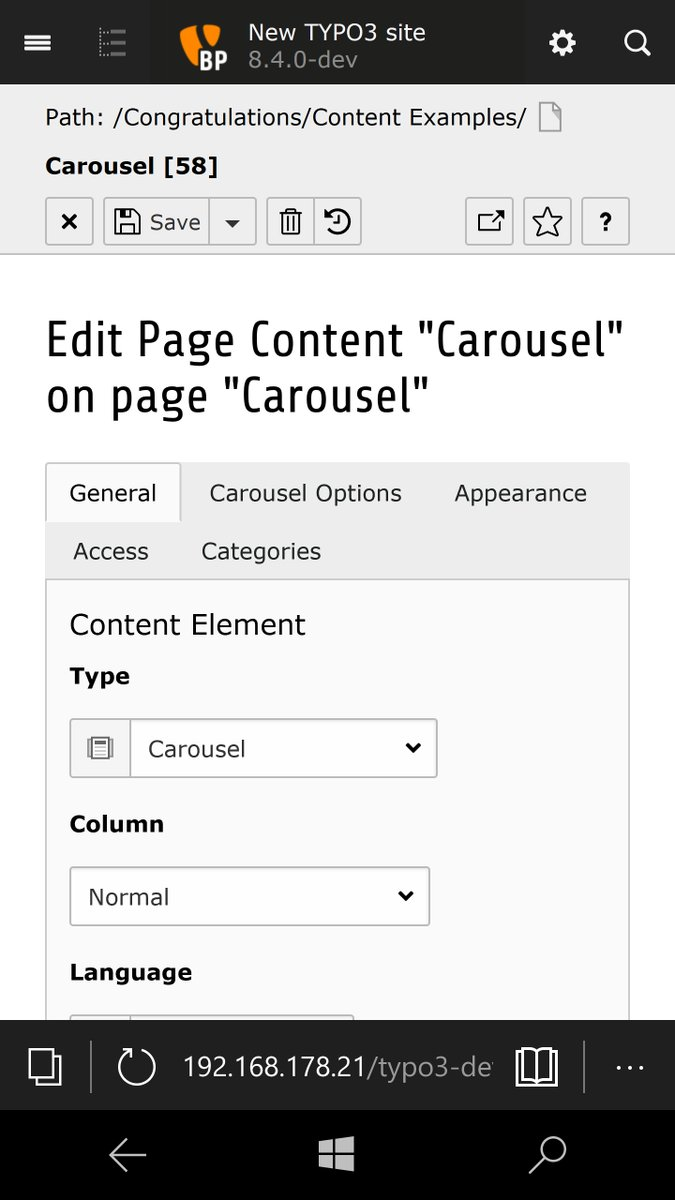
\includegraphics[width=0.25\linewidth]{BackendUserInterface/mobile-responsive-backend.jpg}
	\end{figure}

\end{frame}

% ------------------------------------------------------------------------------
% LTXE-SLIDE-START
% LTXE-SLIDE-UID:		5575ab5c-dea16f71-9f1042a9-fe909828
% LTXE-SLIDE-ORIGIN:	f6668b2d-8932a470-5b9c024c-e4e9f53a English
% LTXE-SLIDE-TITLE:		Install Tool: Upgrade Analysis
% ------------------------------------------------------------------------------

\begin{frame}[fragile]
	\frametitle{Interfaz de Usuario de Backend}
	\framesubtitle{Herramienta de Instalación: Análisis de actualización}

% The install tool, which is also a heavily used feature during updates between
% TYPO3 versions, has received some more beauty, basically finding all documented
% changes with a cool filter to show what is relevant for an integrator,
% extension author or site owner. Although this is already pretty cool, stay
% tuned for even better features to make migrations even easier between TYPO3
% versions!
% The migration and deprecation of existing options and switching within the TCA
% definitions we have in place since TYPO3 v7, is also visible in the Install Tool
% now.

	Las actualizaciones de versión de TYPO3 se han vuelto más fáciles con la nueva herramienta de
	\textbf{Análisis de Actualización} en la Herramienta de Instalación (encontrar/filtrar cambios documentados entre versiones).

	\begin{figure}
		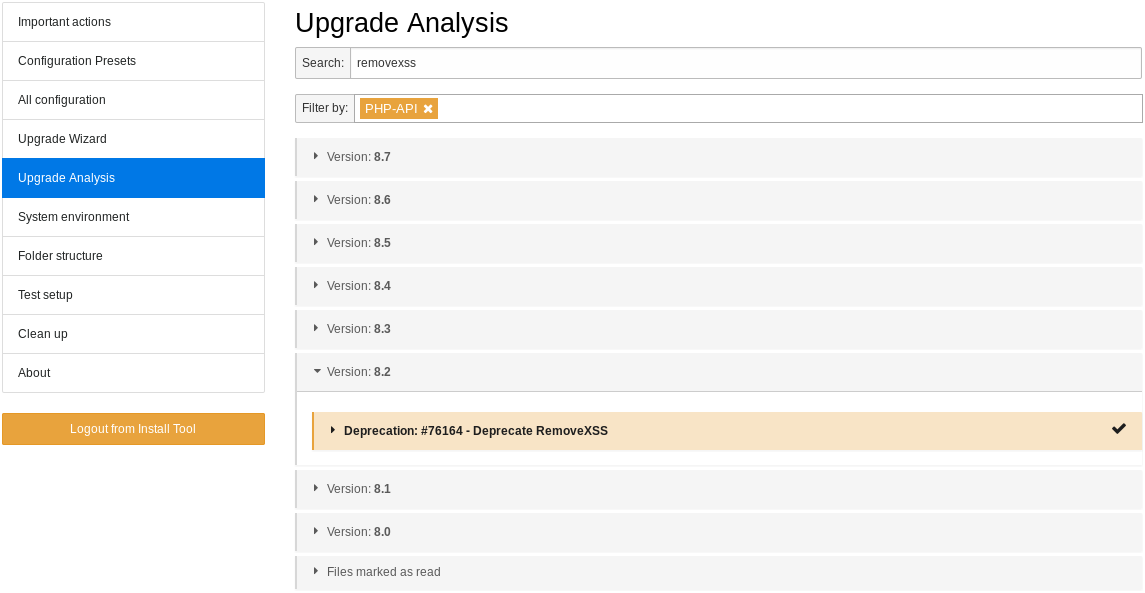
\includegraphics[width=0.45\linewidth]{BackendUserInterface/install-tool-upgrade-analysis.png}
	\end{figure}

\end{frame}

% ------------------------------------------------------------------------------
% LTXE-SLIDE-START
% LTXE-SLIDE-UID:		50104f16-b2e4bddf-13018230-04e5924a
% LTXE-SLIDE-ORIGIN:	9702aaf4-f02bbc35-67902b2e-42855506 English
% LTXE-SLIDE-TITLE:		Install Tool: Upgrade Analysis
% LTXE-SLIDE-REFERENCE:	#78222: Dump Class Loading Information UI in Install Tool
% ------------------------------------------------------------------------------

\begin{frame}[fragile]
	\frametitle{Interfaz de Usuario de Backend}
	\framesubtitle{Herramienta de Instalación: Volcar Información de Autoload}

	Para regenerar la información la información de carga de clases, se ha añadido una nueva acción a la Herramienta de Instalación para volcar la información de autocarga.

	\begin{figure}
		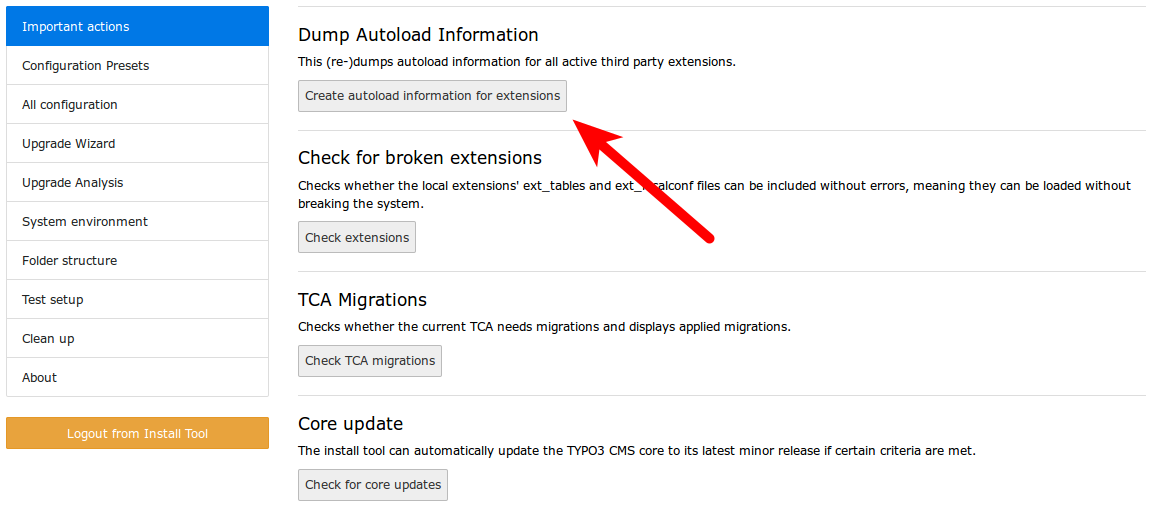
\includegraphics[width=0.8\linewidth]{BackendUserInterface/78222.png}
	\end{figure}

\end{frame}

% ------------------------------------------------------------------------------
% LTXE-SLIDE-START
% LTXE-SLIDE-UID:		50085155-adcb313d-ea111bea-24256edd
% LTXE-SLIDE-ORIGIN:	5a194e82-8eac7f1b-ef2730da-61d781b2 English
% LTXE-SLIDE-TITLE:		Install Tool: TCA Migration Messages
% LTXE-SLIDE-REFERENCE:	#77799: Display TCA migration messages in Install Tool
% ------------------------------------------------------------------------------

\begin{frame}[fragile]
	\frametitle{Interfaz de Usuario de Backend}
	\framesubtitle{Herramienta de Instalación: Mensajes de Migración de TCA}

	En la Herramienta de Instalación se pueden comprobar/listar mensaje/s sobre la migración del TCA.

	\begin{figure}
		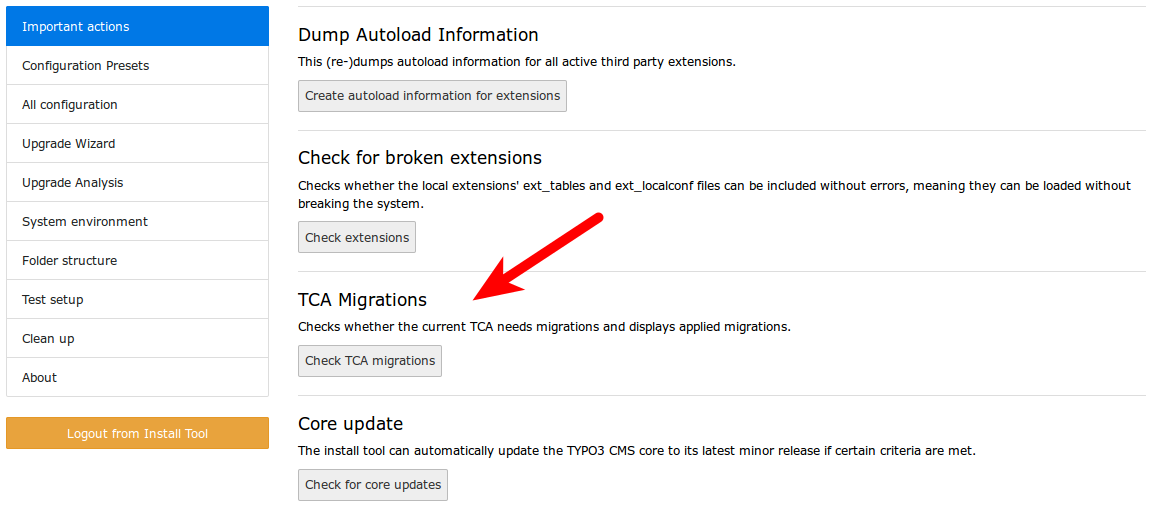
\includegraphics[width=0.8\linewidth]{BackendUserInterface/77799.png}
	\end{figure}

\end{frame}

% ------------------------------------------------------------------------------
% LTXE-SLIDE-START
% LTXE-SLIDE-UID:		96c2ff95-ad3d6444-e8a0f08c-4414281c
% LTXE-SLIDE-ORIGIN:	1e11eae3-872938ec-9612c092-444c408a English
% LTXE-SLIDE-TITLE:		sys_language records are sortable now
% LTXE-SLIDE-REFERENCE:	#77652: Make sys_language records sortable
% ------------------------------------------------------------------------------

\begin{frame}[fragile]
	\frametitle{Interfaz de Usuario de Backend}
	\framesubtitle{Registros \texttt{sys\_language}}

	Para mejorar la usabilidad, se pueden ordenar los registros \texttt{sys\_language}.

	\begin{figure}
		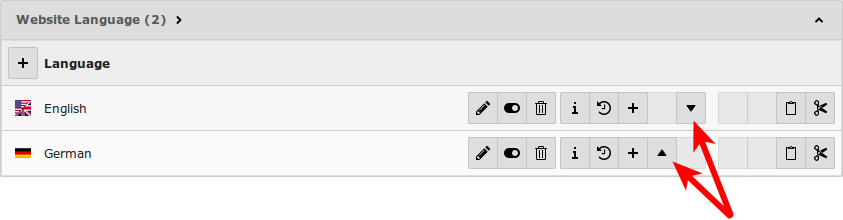
\includegraphics[width=0.8\linewidth]{BackendUserInterface/77652.png}
	\end{figure}

\end{frame}

% ------------------------------------------------------------------------------
% LTXE-SLIDE-START
% LTXE-SLIDE-UID:		2a80d24a-92bcb8cf-490e3269-038d81a8
% LTXE-SLIDE-ORIGIN:	a82823ff-94b9520f-5e6d6056-95f1a797 English
% LTXE-SLIDE-TITLE:		#77668: Hide table listing below group element
% ------------------------------------------------------------------------------

\begin{frame}[fragile]
	\frametitle{Interfaz de Usuario de Backend}
	\framesubtitle{Listado de Tablas bajo los Elementos Grupo}

	\begin{itemize}

		\item La opción de la configuración TCA \texttt{disable\_controls} del tipo "group"
			tiene un nuevo ajuste \texttt{allowedTables} ahora, que oculta la pista sobre tablas permitidas
			a ser referenciadas en el campo "group".

	\end{itemize}

	\begin{figure}
		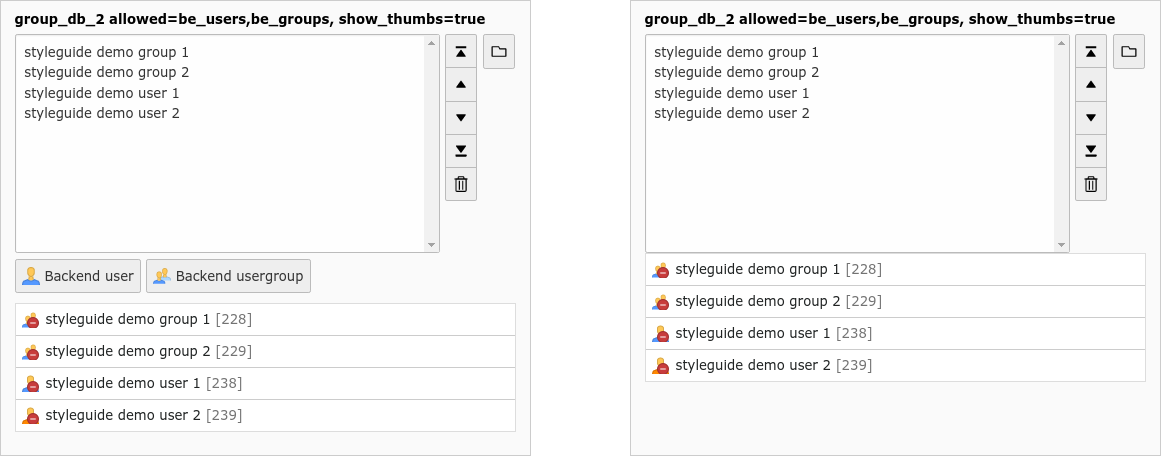
\includegraphics[width=0.85\linewidth]{BackendUserInterface/77668.png}
	\end{figure}

\end{frame}

% ------------------------------------------------------------------------------
